\problemname{Fjarflutningur}

Hin nýlega stofnaða Fjarflutningsstofnun Íslands mun gjörbylta samgöngum á
landinu. Stofnunin hefur sett fram tillögur um hvernig hægt sé að setja upp
orkusparandi fjarflutningskerfi á Íslandi og gera þar með bíla, strætisvagna og
jafnvel flugvélar úreltar. Ríkinu hefur nú verið gert að grannskoða þessa
tillögu, og hefur það haft samband við færustu forritara Íslands til að fá
aðstoð. Hér kemur þú inn í myndina.

Þér hefur verið úthlutað mynd af fjarflutningskerfinu til skoðunar.
Fjarflutningskerfið samanstendur af $N$ fjarflutningsgáttum á mismunandi stöðum
um landið. Hver gátt $a$ hefur ákveðna gátt $b$ sem áfangastað. Þetta þýðir að
í hvert sinn sem maður gengur inn í gátt $a$, þá kemur maður út fyrir framan
gátt $b$. Athugaðu samt að ef maður fer svo inn í gátt $b$, þá þarf maður ekki
endilega að koma aftur út fyrir framan gátt $a$. Hugmynd Fjarflutningsstofnunar
Íslands er að fólk byrjar að fara inn í eina fjarflutningsgátt, fara svo inn í
gáttina sem þau koma út um, og endurtaka þetta svo þar til þau eru komin á
áfangastað.

Ríkið vill nú vita fyrir mismunandi upphafs- og endagáttir $a$ og $b$ hversu
oft maður þarf að ganga inn í gátt til að komast frá $a$ til $b$, eða hvort það
sé einfaldlega ekki hægt. Vinsamlegast svaraðu, fyrir hverja fyrirspurn, hversu
oft þarf að ganga inn í gátt til að komast frá $a$ til $b$, eða $-1$ ef það er
ekki hægt.

Hjálpaðu ríkinu!

\section*{Inntak}
Á fyrstu línu af inntakinu er heiltala $N$ sem táknar fjölda gátta í
fjarflutningskerfinu. Svo fylgja $N$ línur með heiltölu $1 \leq d_i \leq N$ sem
táknar að ef maður fer inn um gátt $i$, þá kemur maður út um gátt $d_i$.
Gáttirnar eru númeraðar frá einum (lægsta hefur númerið $1$, hæsta hefur
númerið $N$), og koma þær í röð frá $1$ til $N$ í inntakinu.

Síðan fylgir lína með heiltölu $Q$ sem táknar fjölda fyrirspurna sem þarf að
svara. Svo fylgja $Q$ línur með tveimur heiltölum $1 \leq s, e \leq N$. Þessar
tölur tákna upphafsgáttina $s$ og endagáttina $e$, og ykkar verkefni er að
svara hversu oft þarf að fara inn í gátt til að komast í gátt $e$ ef byrjað er
í gátt $s$. Í hverri fyrirspurn mun gilda að $s \neq e$.

\section*{Úttak}
Skrifið út $Q$ línur, eina fyrir hverja fyrirspurn: hversu oft maður þarf að
fara inn í gátt til að komast frá upphafsgáttinni til endagáttarinnar. Ef það
er ekki hægt, skrifið út $-1$. Hvert svar á að skrifa á sér línu.

\section*{Útskýring á sýnidæmi}

\begin{figure}[ht!]
\centering
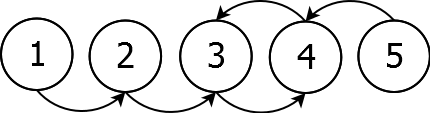
\includegraphics[width=0.4\textwidth]{portaler.png}
\caption{Mynd sem táknar fyrsta sýnidæmið.}
\label{overflow}
\end{figure}

Fjarflutningskerfið í sýnidæminu er sýnt í myndinni að ofan. Við fáum þrjár
fyrirspurnir. Í fyrstu er spurt hversu oft þarf að fara inn í gátt ef maður
byrjar við gátt $1$ og vil komast í gátt $2$. Þar sem maður kemur út um gátt
$2$ þegar maður fer inn í gátt $1$, þá er svarið $1$. Til að fara frá gátt $1$
til $4$ þarf maður að fara inn í gátt þrisvar sinnum. Fyrir síðustu
fyrirspurnina er svarið $-1$, því maður kemst aldrei frá gátt $2$ til $5$ sama
hversu oft maður fer inn í gátt.

\section*{Stigagjöf}
Lausnin mun verða prófuð á miserfiðum inntaksgögnum, og er gögnunum skipt í
hópa eins og sýnt er í töflunni að neðan. Lausnin mun svo fá stig eftir því
hvaða hópar eru leystir.

\begin{tabular}{|l|l|l|l|}
\hline
Hópur & Stig & Inntaksstærð & Önnur skilyrði\\ \hline
1     & 10         & $ 1 \le N \le 1\,000,\ 1 \le Q \le 1\,000$ & Það er alltaf hægt að komast frá upphafsgáttinni til endagáttarinnar.\\ \hline
2     & 20         & $ 1 \le N \le 1\,000,\ 1 \le Q \le 1\,000$ &  \\ \hline
3     & 10         & $ 1 \le N \le 7\,000,\ 1 \le Q \le 120\,000$ & Það er alltaf hægt að komast frá upphafsgáttinni til endagáttarinnar.\\ \hline
4     & 10         & $ 1 \le N \le 7\,000,\ 1 \le Q \le 120\,000$ &  \\ \hline
5     & 10         & $ 1 \le N \le 50\,000,\ 1 \le Q \le 70\,000$ & Það er alltaf hægt að komast frá upphafsgáttinni til endagáttarinnar. Prófin eru líka aðeins léttari en í hópi 6.\\ \hline
6     & 30         & $ 1 \le N \le 50\,000,\ 1 \le Q \le 70\,000$ & Það er alltaf hægt að komast frá upphafsgáttinni til endagáttarinnar. \\ \hline
7     & 10         & $ 1 \le N \le 50\,000,\ 1 \le Q \le 70\,000$ &  \\ \hline
\end{tabular}
